\section{Image}
Image data is frequently used in various forms within the PixelLight framework. \ac{GUI} images, renderer textures and so on, all those are using the image class of PLGraphics to load in the data in one of the many supported image file formats or saving the data.

The image class may look quite complex on the first look, but using it is... now, look for yourself:

\begin{lstlisting}[caption=Image usage]
// Image instance
PLGraphics::Image cImage;

// Load an image
if (cImage.LoadByFilename("MyImage.png")) {
	// Get a pointer to the image buffer
	PLGraphics::ImageBuffer *pImageBuffer = cImage.GetBuffer();
	if (pImageBuffer && pImageBuffer->GetDataFormat() == PLGraphics::DataByte) {
		// Get a pointer to the image data
		PLCore::uint8 *pData = pImageBuffer->GetData();

		// Loop through the hole image data and mess it up
		for (PLCore::uint32 i=0; i<pImageBuffer->GetDataSize(); i++, pData++)
			*pData = ((*pData) + i) % 255;

		// Save the manipulated image
		cImage.SaveByFilename("MyManipulatedImage.png");
	}
}
\end{lstlisting}




\subsection{Mipmaps}
Mipmaps are the same image - but in multiple resolutions.\footnote{Although it's also possible to put a totally different image into each of the mipmaps}

Mipmaps are usually used for textures to improve the performance and the visual quality.
Within PLRenderer: If a texture is allowed to use mipmapping, mipmaps are created automatically if the loaded texture doesn't provide such information. Image formats like dds can provide predefined mipmap information. In this case, you have to define all mipmap levels down to 1x1 otherwise the texture is invalid when you try to use any min filter that uses mipmaps. OpenGL normally uses white color when invalid/incomplete texture is enabled.




\subsection{Compression}
The image system supports holding a compressed version of the image data. Supported compression formats are DXT1, DXT3, DXT5, ATI1N and ATI2N (marketing name: 3Dc).

The main usage is for texture compression. If a texture is allowed to use compression, the image is compressed by the renderer automatically if the loaded texture doesn't provide such information. Image formats like dds can provide compressed image information. In this case, the renderer will use this compressed data instead compressing automatically. Because the image system is only decompressing image data when really required, loading of compressed textures is quite fast!




\subsection{Cube Maps}
Cube maps are a special type of an image. In fact a cube map is build up of 6 different images - one for each cube side with the same dimensions. The cub map itself is used like the other normal images.

You can for example use the dds file format to load in cube maps.

The main usage is for textures. Cube textures are useful for
\begin{itemize}
\item{As a texture: Cube map reflections}
\item{As a texture: A normalization cube map can be used within fragment shaders to normalize vectors faster\footnote{But with less quality and on modern hardware it may not be faster}}
\end{itemize}




\subsection{3D Images}
Besides 2D images, the image system does also support 3D images. 3D images can be seen as a stack of 2D images.

The main usage is for textures. A 3D texture is mapped into (s, t, r = u, v, w = x, y, z) coordinates such that it's lower left back corner is (0 ,0, 0) and it's upper right front corner is (1, 1, 1).

\begin{figure}
  \begin{center}
    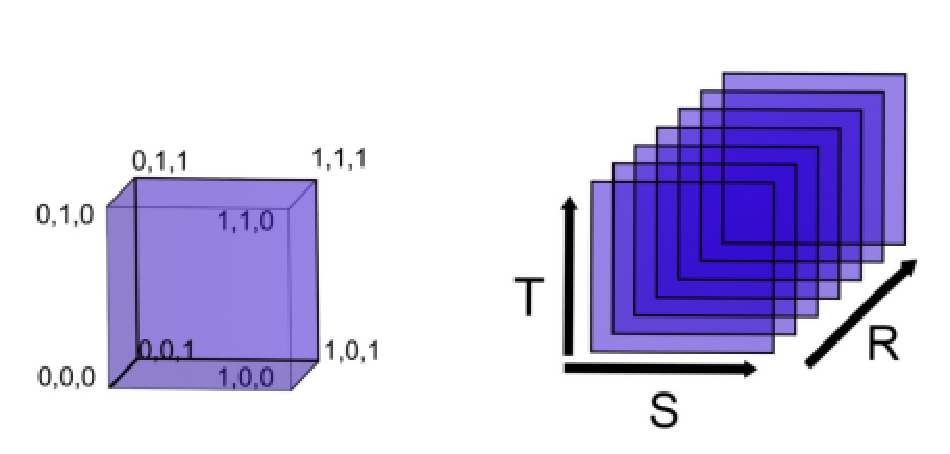
\includegraphics{pics/3DTex_1.eps}
  \end{center}
  \caption{3D texture}
  \label{fig:3D texture}
\end{figure}

3D textures are useful for

\begin{itemize}
\item{Volume rendering and examining a 3D volume one slice at a time}
\item{Animating textured geometry, for example, people that move}
\item{Eliminating distortion effects that occur when you try to map a 2D image onto 3D geometry}
\item{Solid texturing, for example, wood, marble and so on}
\end{itemize}

Texel values defined in a 3D coordinate system form a texture volume. You can extract textures from this volume by intersecting it with a plane oriented in 3D space, as shown below.

\begin{figure}
  \begin{center}
    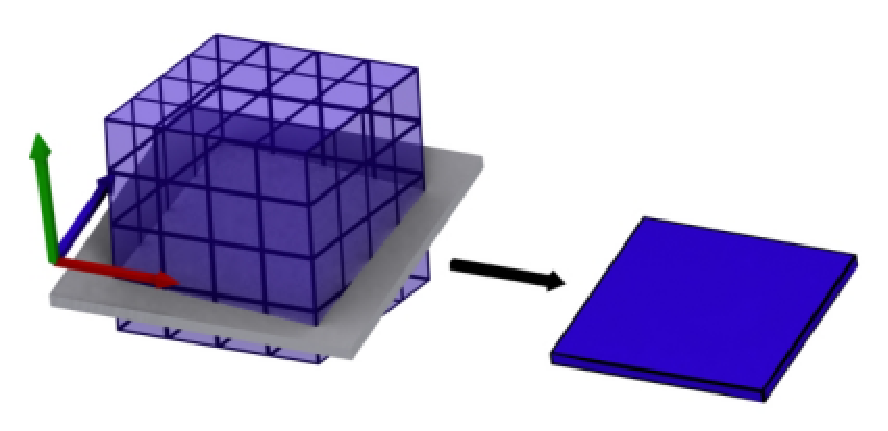
\includegraphics{pics/3DTex_2.eps}
  \end{center}
  \caption{3D texture}
  \label{fig:Extracting a Planar Texture From a 3D Texture Volume}
\end{figure}

The resulting texture, applied to a polygon, is the intersection of the volume and the plane. The orientation of the plane is determined from the texture coordinates of the vertices of the polygon.
